\chapter{Theoretische Grundlagen}
\label{chap:theoretische_grundlagen}
\section{Greensche Funktionen}
Die Greensche Funktion ist für zwei Operatoren mit der zetlichen Entwicklung 
\begin{equation}
    A \left ( \tau \right ) = \symup{e}^{H \tau} A_\text{S} \symup{e}^{-H \tau}  \label{eqn:heisenbergpic}
\end{equation}
definiert als 
\begin{align}
    G_{A,B} \left (\tau, \tau' \right ) &= - \frac{1}{\hbar} \langle T_s \left ( A \left (\tau \right ) B \left ( \tau' \right ) \right ) \rangle \\
    & = - \frac{1}{\hbar} \left(  \langle A \left (\tau \right ) B \left ( \tau' \right ) \rangle \symup{\Theta} \left ( \tau - \tau' \right) + s 
    \langle B \left ( \tau' \right ) A \left (\tau \right ) \rangle \symup{\Theta} \left ( \tau' - \tau \right)  \right ) \; \text{,} \label{eqn:greensfunction}
\end{align}
wobei $H$ der Hamiltonoperator, $A_\text{S}$ ein Operator im Schöringerbild, $T_s$ der Zeitordnungsoperator, 
$\langle \ldots \rangle$ ein Erwartungswert und $\symup{\Theta} \left ( \tau' - \tau \right)$ die Heaviside-Funktion ist.\cite{greensfunction}
Der Parameter $s$ sorgt mit $s=+1$ für bosonische bzw. $s=-1$ für fermionische Operatoren für das richtige Vorzeichen.
Der Erwartungswert ist bezüglich der großkanonischen Gesamtheit durch 
\begin{equation*}
    \langle \ldots \rangle = \frac{1}{Z} \text{Sp}(\symup{e}^{-\beta H} \ldots)
\end{equation*}
gegeben.\cite{greensfunction}
Die Zustandssumme $Z$ stellt dabei einen Normierungsfaktor dar.
%Die imaginäre Zeit $\tau$ ist über die reale Zeit $t$ als $\tau = it$ definiert.
In Gleichung \eqref{eqn:heisenbergpic} wurde das reduzierte Planksche Wirkungsquantum breits auf eins gesetzt, was in den folgenden Abschnitten beibehalten wird.
Da in dieser Arbeit nur fermionische Systeme betrachtet werden, wird $s$ ab jetzt ohne weitere Bemerkungen auf $-1$ gesetzt.
Unter der Annahme, dass die partielle Ableitung von $A$ verschwindet, ist die zeitliche Entwicklung eines Operators 
$A$ durch die Heisenbergsche Bewegungsgleichung gemäß 
\begin{equation}
\frac{\symup{d}}{\symup{d}t} A \left (\tau \right ) = \symup{i}  [H, A] \iff \frac{\symup{d}}{\symup{d}\tau} A \left (\tau \right ) = [H, A] \label{eqn:heisenbergeom}
\end{equation}
gegeben.
In dieser Arbeit ist die Bewegungsgleichung für die Greensche Funktion \eqref{eqn:greensfunction} von großer Bedeutung, welche mittels 
partieller Ableitung nach der Zeit gewonnen werden kann.\cite{greensfunction}
Somit folgt
\begin{align*}
    \begin{split}
    \frac{\partial}{\partial \tau} G_{A,B} \left (\tau, \tau' \right) = 
    &- \left \langle \frac{\partial}{\partial \tau}A \left (\tau \right ) B \left ( \tau' \right ) \right \rangle
    \symup{\Theta} \left ( \tau - \tau' \right) -  \langle A \left (\tau \right ) B \left ( \tau' \right ) \rangle \symup{\delta} \left ( \tau - \tau' \right)\\
    &+ \left \langle B \left ( \tau' \right ) \frac{\partial}{\partial \tau}A \left (\tau \right ) \right \rangle \symup{\Theta} \left ( \tau' - \tau \right)
    -  \langle B \left ( \tau' \right ) A \left (\tau \right ) \rangle \symup{\delta} \left ( \tau' - \tau \right)
    \end{split}
    \\[2ex]
    \begin{split}
    = &- \left \langle [H,A] B \left ( \tau' \right ) \right \rangle
    \symup{\Theta} \left ( \tau - \tau' \right) -  \langle A \left (\tau \right ) B \left ( \tau' \right ) \rangle \symup{\delta} \left ( \tau - \tau' \right)\\
    &+ \left \langle B \left ( \tau' \right ) [H,A] \right \rangle \symup{\Theta} \left ( \tau' - \tau \right)
    -  \langle B \left ( \tau' \right ) A \left (\tau \right ) \rangle \symup{\delta} \left ( \tau' - \tau \right)
    \end{split}
    \\[2ex]
    =\; & G_{[H,A],B}(\tau, \tau') - \langle [A,B] \rangle \symup{\delta} \left ( \tau - \tau' \right) \; \text{.}
\end{align*} 
Dabei ist  $\symup{\delta} (\tau-\tau') = \symup{\delta} (\tau'-\tau) $ die Deltadistribution, welche durch Ableitung der Heaviside-funktion gewonnen werden kann.
In der dritten Zeile wurde die Heisenbergsche Bewegungsgleichung \eqref{eqn:heisenbergeom} ausgenutzt.
Um eine einfachere Form der Bewegungsgleichung für die Greensche Funktion zu erhalten, wird diese fourier-transformiert.
Somit ergibt sich die Bewewgungsgleichung zu 
\begin{equation}
    zG_{A,B}(z) = \langle \{A,B\} \rangle - G_{[H,A],B}(z) \; \text{,} \label{eqn:fouriereom}
\end{equation} 
wobei der $\{ A,B \} = AB+BA$ der Antikommutator ist.\cite{greensfunction}
Eine wichtige Eigenschaft der Greenschen Funktion ist die Linearität, aus welcher mit $\alpha, \beta \in \mathbb{C}$
\begin{equation*}
    G_{(\alpha A + \beta B), C} = \alpha G_{A,C} + \beta G_{B,C}
\end{equation*}
folgt.

\section{Tight Binding Modell}
\label{sec:tightbinding}
In der Tight Binding Näherung wird von stark gebundenen, lokalisierten Elektonen ausgegangen.\cite{Czycholl}
Dazu wird der volle Hamiltonian eines Elektrons im Festkörper
\begin{equation}
    H = \frac{\vec{p}^2}{2m} + \sum_{i\alpha} v(\vec{r}-\vec{l}_i - \vec{R}_{\alpha}) = \frac{\vec{p}^2}{2m} + v_{\vec{R}}(\vec{r})\label{eqn:electron_hamiltonian}
\end{equation}
betrachtet.\cite{Czycholl}
Der Vektor $\vec{R}_{\alpha}$ ist die Position innerhalb der Basis $\alpha$ in der Einheitszelle mit dem Gittervektor $\vec{l}_i$.
Mitels des Wellenvektors $\vec{k}$ lassen sich aus den atomaren Wellenfunktionen $\Psi_{lm} \left (\vec{r}-\vec{l}_i - \vec{R}_{\alpha} \right )$ mit $l$ und $m$ als Drehimpulsquantenzahlen
Blochzustände
\begin{equation}
    \Psi^{\alpha}_{lm}(\vec{k}, \vec{r}) = \frac{1}{\sqrt{N}} \sum_{i} \symup{e}^{\symup{i}\vec{k}\vec{l}_i} \Psi_{lm}(\vec{r}-\vec{l}_i - \vec{R}_{\alpha}) 
\end{equation}
konstuieren, welche die Gitterperiodizität besitzen.\cite{SC_literature}
Für die Tight Binding Modellierung sind die Matrixelemente des Hamiltonians \eqref{eqn:electron_hamiltonian}
relevant, welche in der Blochbasis durch
\begin{equation*}
    \bra{\Psi^{\alpha}_{lm}} H \ket{\Psi^{\alpha'}_{l'm'}} = \varepsilon_{lm,l'm'}^{\alpha \alpha'} \braket*{\Psi^{\alpha}_{lm}}{\Psi^{\alpha'}_{l'm'}}
    - \frac{1}{N} \sum_{i\alpha \neq i' \alpha'} \symup{e}^{\symup{i}\vec{k}(\vec{l}_{i'}-\vec{l}_{i})}  t^{i\alpha,i'\alpha'}_{lm,l'm'}
\end{equation*}
gegeben sind.\cite{SC_literature}\cite{Czycholl}
Die Orbitalenergien im Kristallfeld sind durch $\varepsilon_{lm,l'm'}^{\alpha \alpha'}$ gegeben.\cite{SC_literature}
Dabei gilt
\begin{equation*}
    t^{i\alpha,i'\alpha'}_{lm,l'm'} = - \int \symup{d}^3r \; \overline{\Psi}_{lm} \left (\vec{r}-\vec{l}_i - \vec{R}_{\alpha} \right ) 
    \left ( v_{\vec{R}} (\vec{r}) - v \left (\vec{r} - \vec{l}_{i'} - \vec{R}_{\alpha'} \right )   \right ) \Psi_{l'm'} \left (\vec{r}-\vec{l}_{i'} - \vec{R}_{\alpha'} \right )  \; ,
\end{equation*}
wobei im stark lokalisierten Fall die Dreizentren-Beiträge vernachlässigt werden können und  
nur noch das Zweizentren-Integral 
\begin{equation*} 
    t^{i\alpha,i'\alpha'}_{lm,l'm'} = - \int \symup{d}^3r \; \overline{\Psi}_{lm} \left (\vec{r}-\vec{l}_i - \vec{R}_{\alpha} \right ) 
    v \left ( \vec{r} - \vec{l}_{i} - \vec{R}_{\alpha} \right ) \Psi_{l'm'} \left (\vec{r}-\vec{l}_{i'} - \vec{R}_{\alpha'} \right ) 
\end{equation*}
übrig bleibt.\cite{SC_literature}
Dieses Zweizentren-Integral ist das für das Tight Binding Modell typische Hüpfmatrixelement.
Damit kann der Tight Binding Hamiltonian in zweiter Quantisierung bei Vernachlässigung der 
magnetischen Quantenzahl $m$ durch
\begin{equation}
    H = - \sum_{ii'} \sum_{\alpha \alpha'}\sum_{ll'} t^{i\alpha,i'\alpha'}_{ll'}  c_{il\alpha}^\dagger c_{i'l'\alpha'}  \label{eqn:tight-binding-hamiltonian}
\end{equation}
angegeben werden.\cite{anders-fkt}
Dabei vernichtet(erzeugt) der Operator $c_{il\alpha}$($c_{il\alpha}^{\dagger}$ ) ein Elektron im Orbital $l$ in der Einheitszelle $i$,
innerhalb der Basis am Platz $\alpha$.
Je nach Modellannahme läuft die Summe dann über z.B. nächste oder übernächste Nachbarn.
\section{Slater-Koster-Integrale}
Jegliche Informationen dieses Abschnitts sind aus \cite{SC_literature} entnommen worden.
Die Slater-Koster-Integrale sind für zwei Orbitale definiert als
\begin{equation}
    E_{lm,l'm'} = \int \symup{d}^3r \; \overline{\Psi}_{lm} (\vec{r}-\vec{d})
    V(\vec{r} - \vec{d}) \Psi_{l'm'} (\vec{r}) \; ,
\end{equation}
worin schon erkenntlich wird, dass diese nur von dem Abstand $\vec{k}$ abhängen.
Hierbei ist $\Psi_{lm}(\vec{r})$ wieder die atomare Wellenfunktion und $V\vec{r}$ das Potential am Ort $\vec{r}$.  
Diese Integrale können wiederrum in einige unabhängige Integrale $V_{ll'\beta}$ zerlegt werden, welche sich durch die Orbitale, $l$ und $l'$, sowie den Bindungen ($\sigma$, $\pi$, $\delta$) unterscheiden.
Als Beispiel würde sich bei dem Überlapp zwischen einem $s$- und $p_x$-Orbital das Integral in zwei 
Slate-Koster-Integrale, $V_{sp\sigma}$ und $V_{sp\pi}$, aufteilen (Abb. \ref{fig:TC}).
\begin{figure}
    \centering
    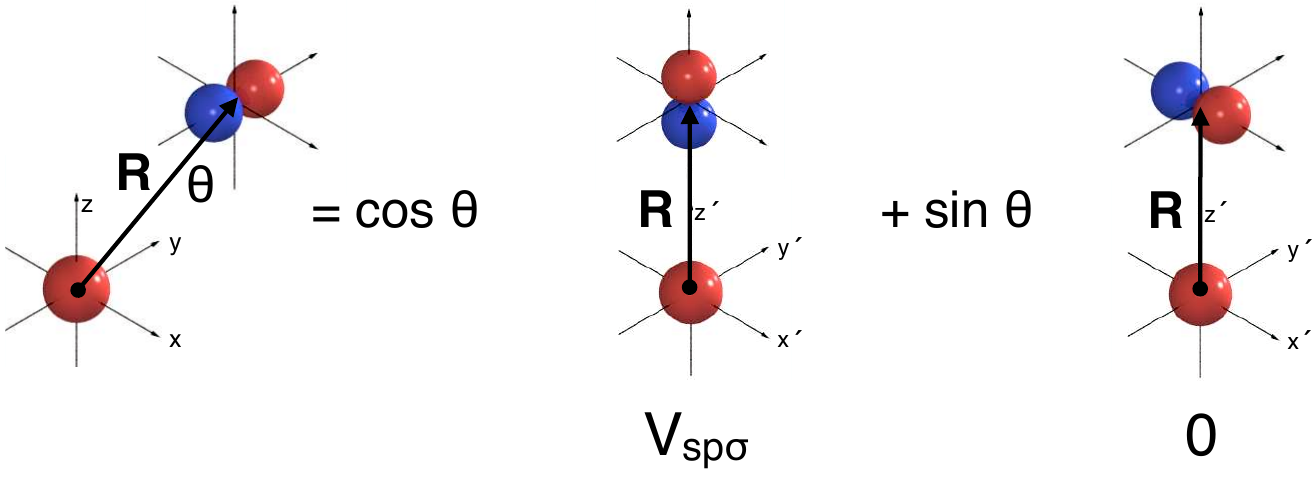
\includegraphics[width = 0.85 \textwidth]{Plots/tc.png}
    \caption{TC}
    \label{fig:TC}
\end{figure}
Das Integral $V_{sp\pi}$ verschwindet in diesem Beispiel aufgrund der Symmetrie.
Jedoch trägt die $\sigma$-Bindung bei, welche